\documentclass[a4paper]{cernatsnote}
\usepackage[utf8]{inputenc}

\usepackage{subcaption}
\usepackage{graphicx}
\usepackage{longtable}
\usepackage{booktabs}
\usepackage{float}

\title{Optics correction in Beam test 2021}
\documentlabel{CERN-ACC-NOTE-2022-YYYY}
\keywords{optics, LHC, beam-test}

\author{ T.~Persson, J.~Dilly, E.~Fol, H.~Garc\'ia Morales, M.~Hofer,
 J.~Keintzel, M.~Le~Garrec, E.H.~Maclean, L.~Malina,  F.~Soubelet, R.~Tom\'as, L.~Van~Riesen-Haupt,  A.~Wegscheider}
\date{February 2022}
%Plots to include:
%comp with old Vertical dispersion
%Comp with old measurement beta-beat
%Second order dispersion
%3D kicks ?
\begin{document}
\maketitle
\begin{abstract}
The LHC beam test in 2021 was aimed at finding potential issues with the machine as well as enable testing of new software and hardware. The optics measurements were all carried out at the injection energy of 450~GeV. The main measurements were: $\beta$-beat, Normalized dispersion and higher order chromaticity measurements but also test of the 3D excitation as well as the feed-down from the MCS to coupling was measured. The initial observation was a large $\beta$-beat but this was explained by a swap of the Q7R3 between Beam~1 and Beam~2. After the swap was fixed the $\beta$-beat was very close to what was measured for the virgin ATS in Run~2. 
\end{abstract}
\section{Linear optics}
The beam test week took place in the autumn of 2021 with the intention of testing the LHC after the LS2 to be ready for the full restart in 2022.
The initial measurement of the $\beta$-beat showed significantly higher values than what was measured previously during commissioning. This is shown in Fig.~\ref{fig:initalVs2016} for Beam~1 and Beam~2 respectively.  


\begin{figure}[ht]
\begin{subfigure}{.5\textwidth}
  \centering
  % include first image
  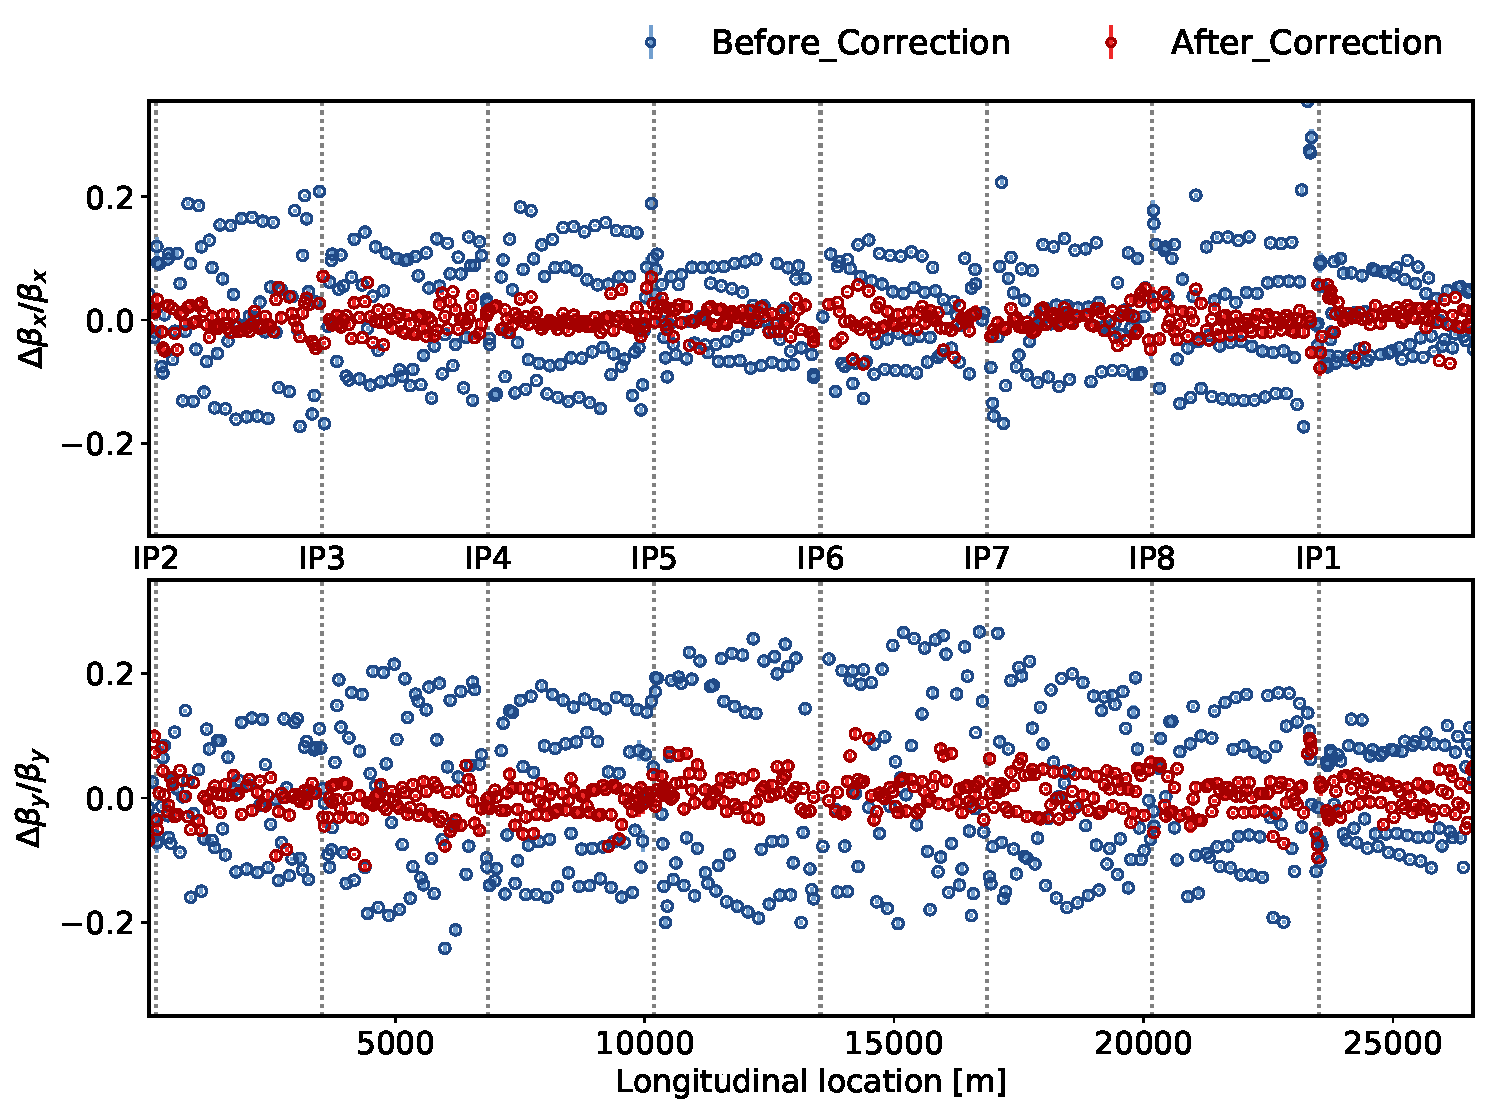
\includegraphics[width=.8\linewidth]{plots/beam1/beta_beat_swapped_vs_2016.pdf}  
  \caption{Beam~1}
  \label{fig:sub-first}
\end{subfigure}
\begin{subfigure}{.5\textwidth}
  \centering
  % include second image
  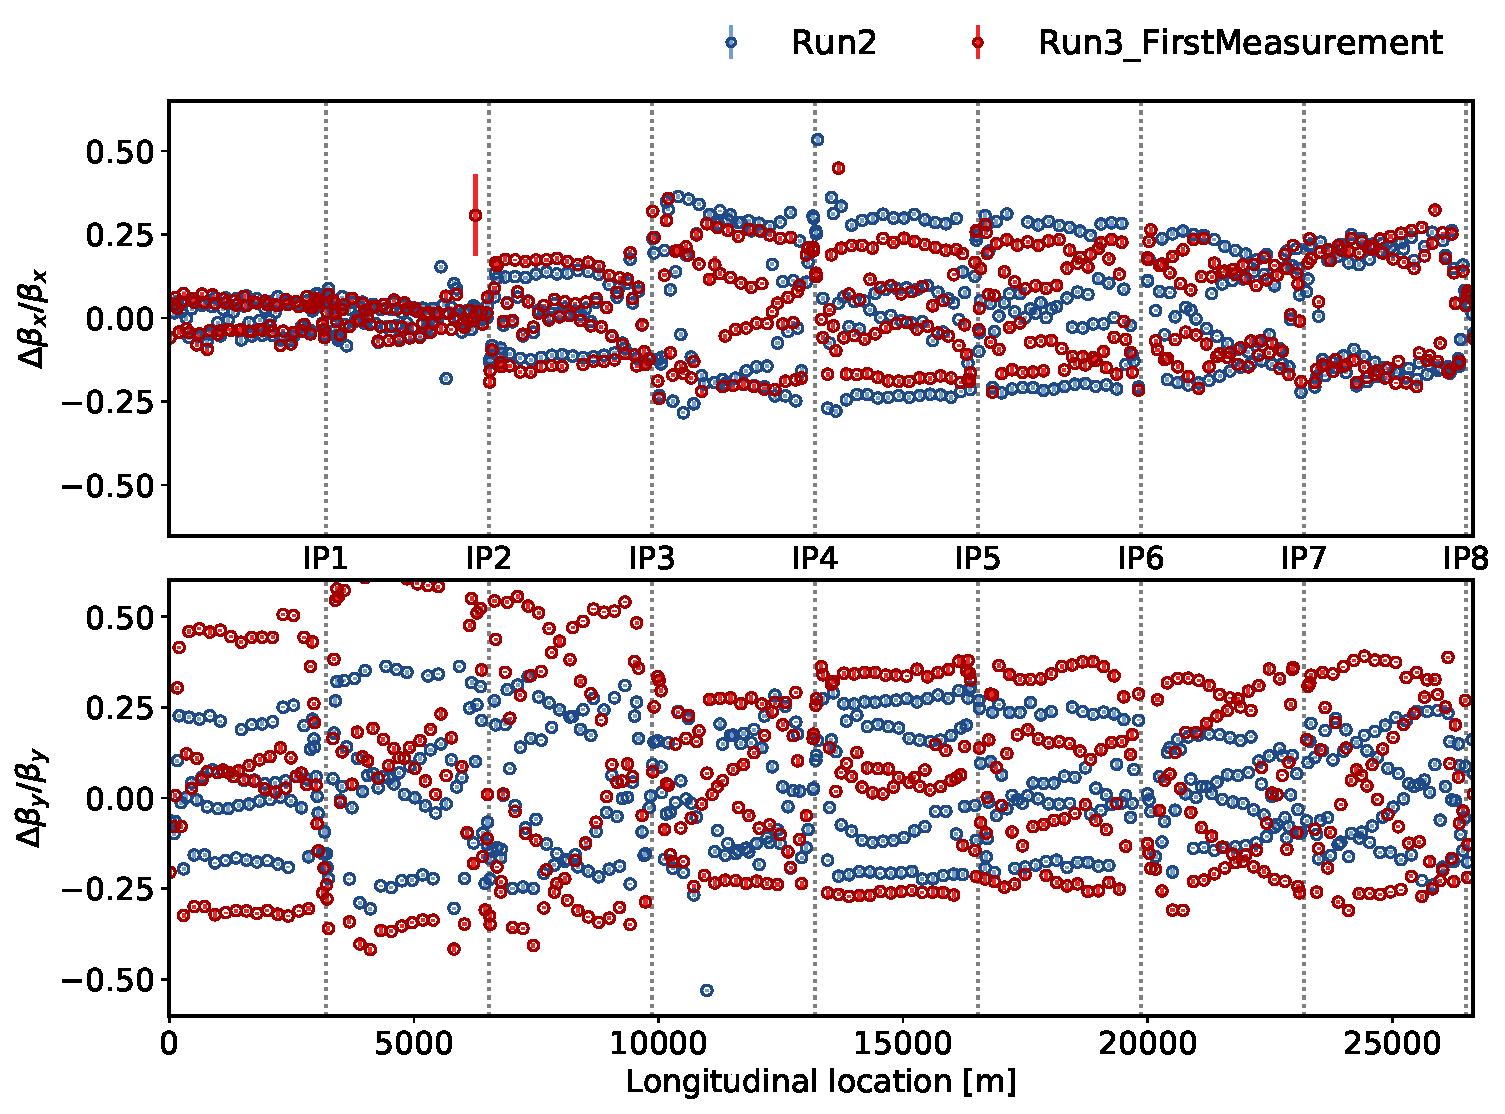
\includegraphics[width=.8\linewidth]{plots/beam2/B2_BetaBeat_2016_vs_first2021.pdf}  
  \caption{Beam~2}
  \label{fig:sub-second}
\end{subfigure}
\caption{The $\beta$-beating for the first measurement in 2021 compared to the measurement in 2016 (during MD).}
\label{fig:initalVs2016}
\end{figure}


The first attempt was to try to understand if something had gone wrong during the pre-cycle or the fact that the machine had been around 40h at injection without any pre-cycle could have an effect. The re-measurement showed a small effect on the $\beta$-beat. After that we attempted to find the location of the error was made. Using the segment-by-segment technique it was found that there was a large phase deviation around IP3 and in particular around IR3Q7. It was decided that we should try to trim on that magnet in order to reduce the $\beta$-beat. The first observation was that nothing changed at all (not even a tune change). We then observed that the tune was changing on the opposite beam. We then repeated the test for the other IR3Q7 and we then again observed a change in tune on the opposite beam. From that we could conclude that indeed the IR3Q7s were swapped. This was then traced to an old swap already detected in Run~1. This was fixed at that time but then during the LS2 it was again re-introduced. After this was corrected on the software side a new measurement was carried out and the $\beta$-beat is shown in Fig.~\ref{fig:before_after_swap}. In this plot we can see that the $\beta$-beat was significantly reduced, as expected, after the swap was corrected.  

\begin{figure}[ht]
\begin{subfigure}{.5\textwidth}
  \centering
  % include first image
  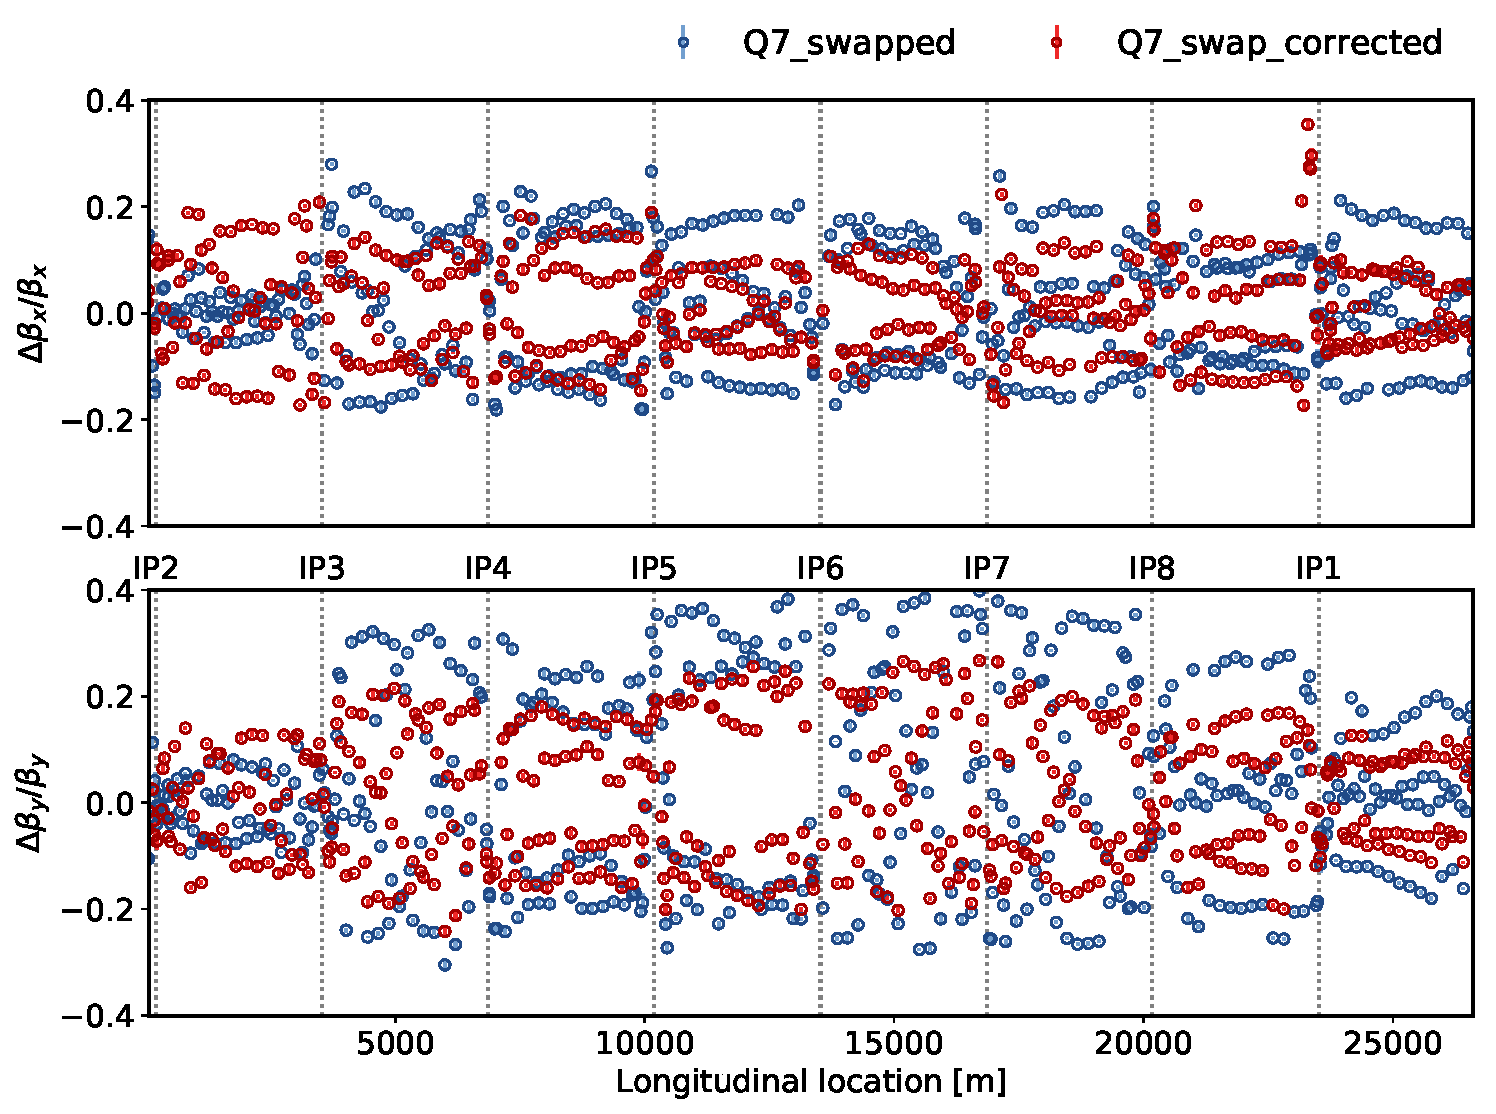
\includegraphics[width=.8\linewidth]{plots/beam1/beta_beat_before_after_swap.pdf}  
  \caption{Beam~1}
  \label{fig:sub-first}
\end{subfigure}
\begin{subfigure}{.5\textwidth}
  \centering
  % include second image
  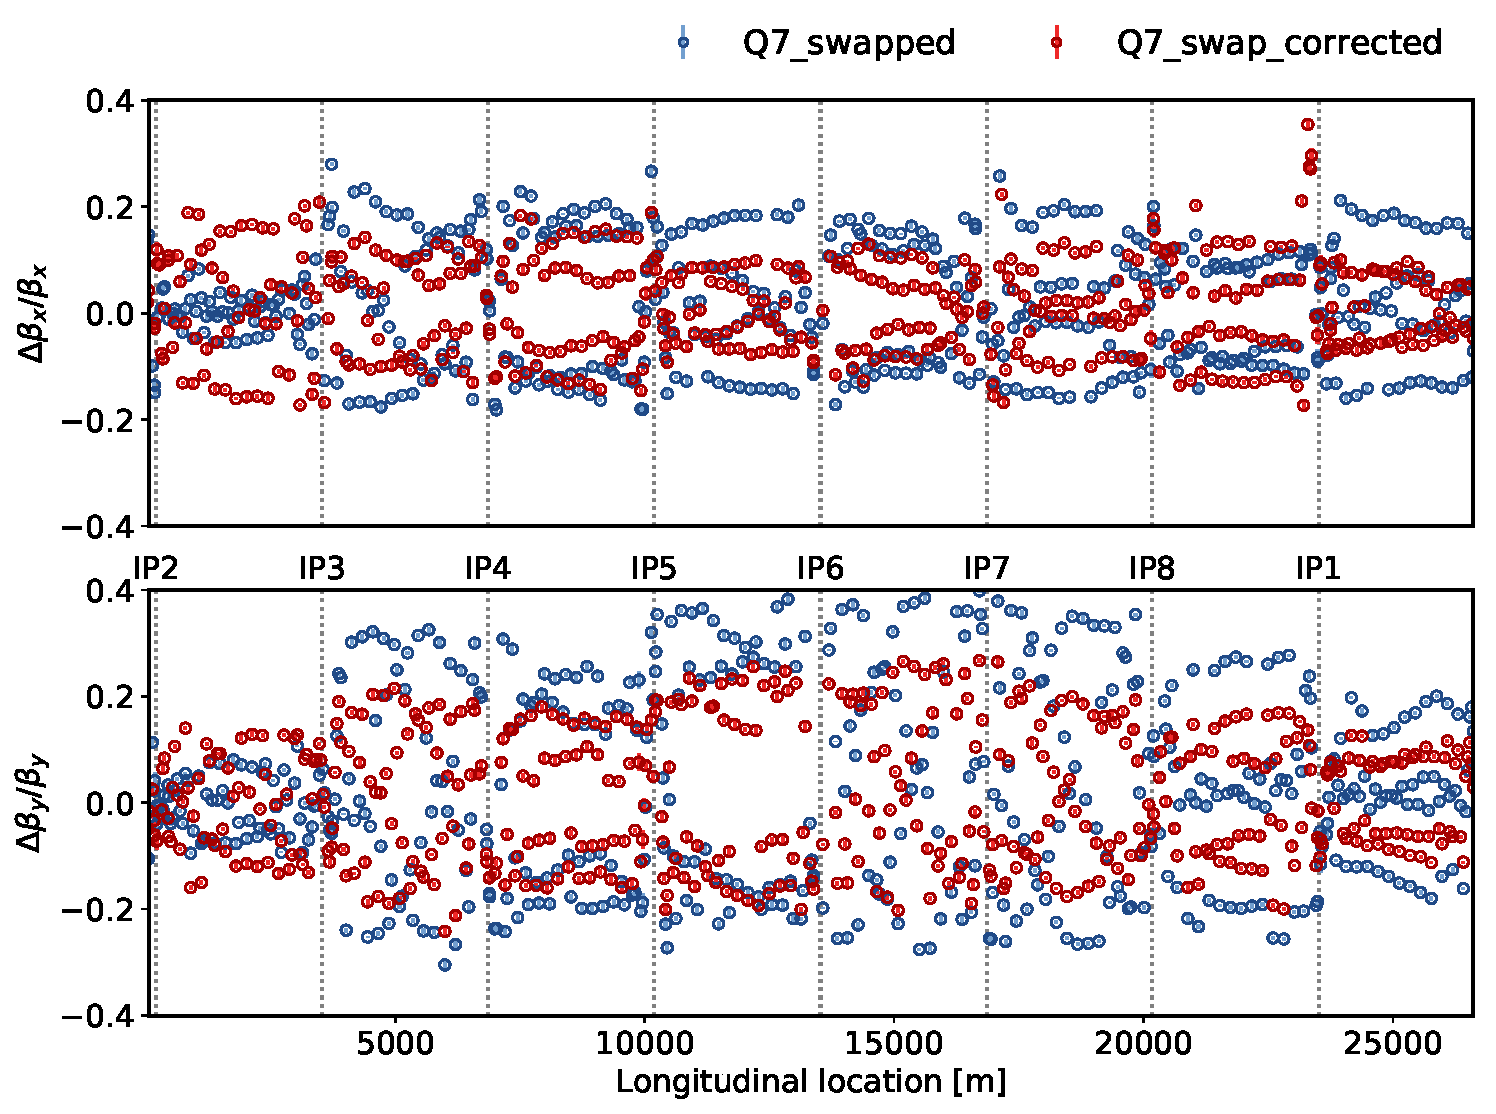
\includegraphics[width=.8\linewidth]{plots/beam1/beta_beat_before_after_swap.pdf}  
  \caption{Beam~2}
  \label{fig:sub-second}
\end{subfigure}
\caption{A comparison of before and after correcting the swap of the Q7R3.}
\label{fig:before_after_swap}
\end{figure}

It is also interesting to observe if there is any sign of any degradation or any other major changes in the machine compared to Run~2. An example of a such comparison is shown in Fig.~\ref{fig:after_swap_vs_2016}. We observe that the $\beta$-beat is similar between the two measurements and the small differences can be explained from the slightly different optics and change of a few of the dipoles. 

\begin{figure}[ht]
\begin{subfigure}{.5\textwidth}
  \centering
  % include first image
  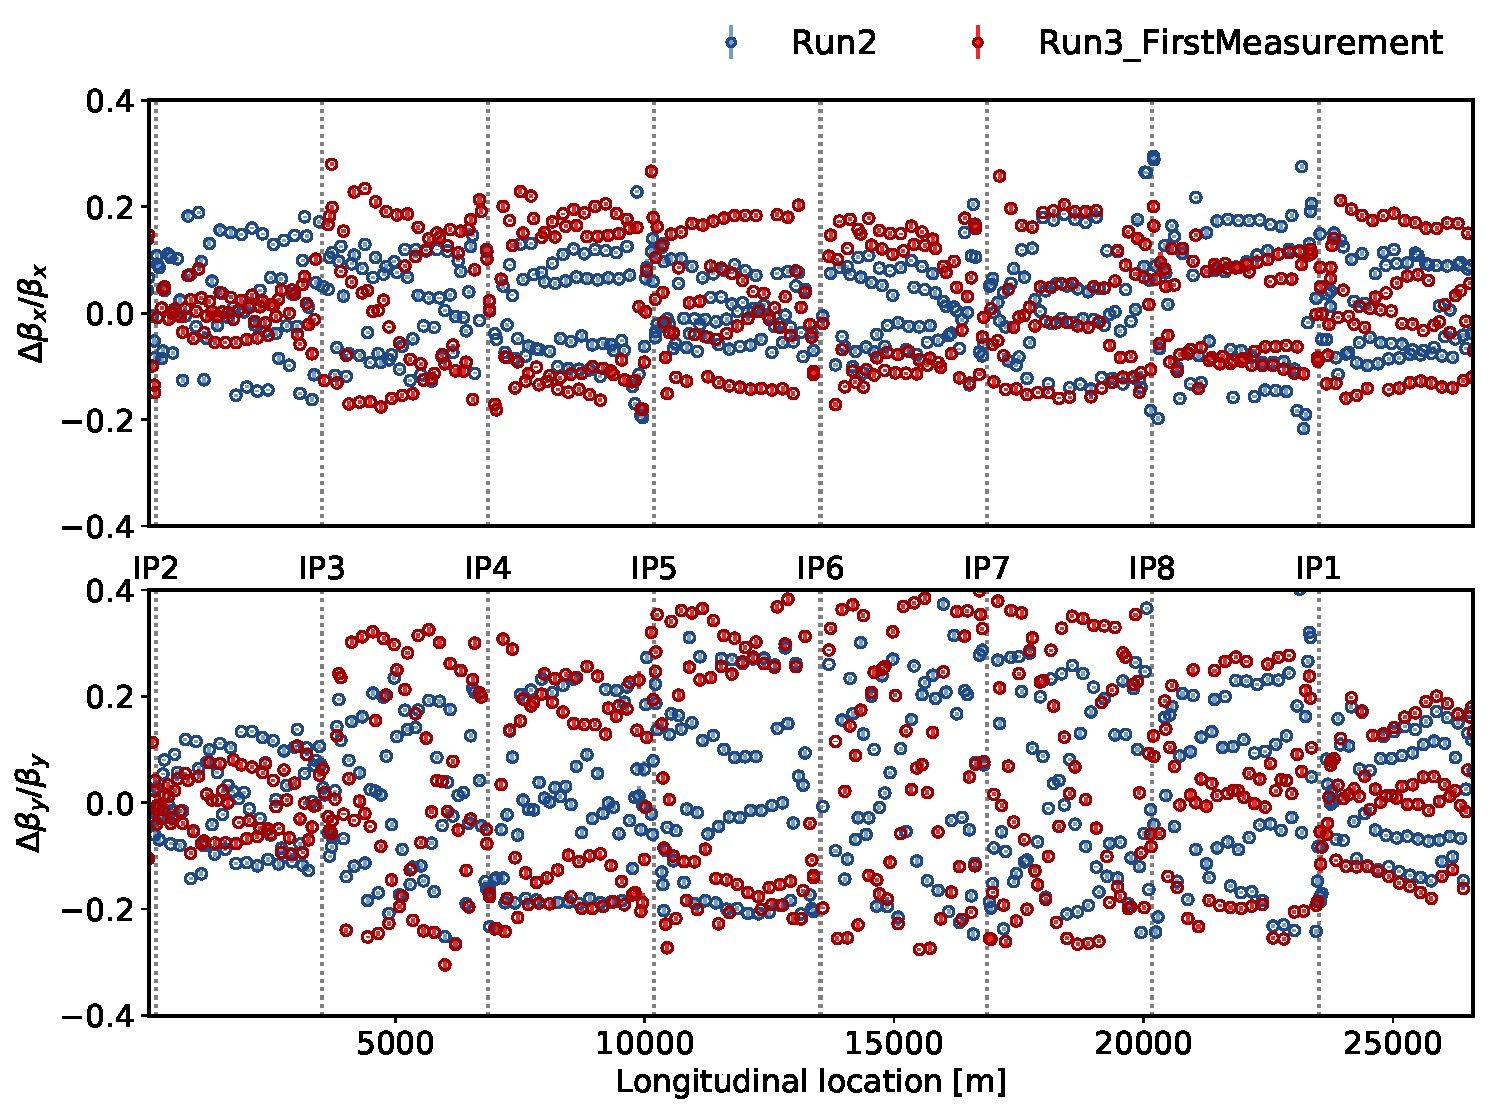
\includegraphics[width=.8\linewidth]{plots/beam1/beta_beat_virgin_2016_2021.pdf}  
  \caption{Beam~1}
  \label{fig:sub-first}
\end{subfigure}
\begin{subfigure}{.5\textwidth}
  \centering
  % include second image
  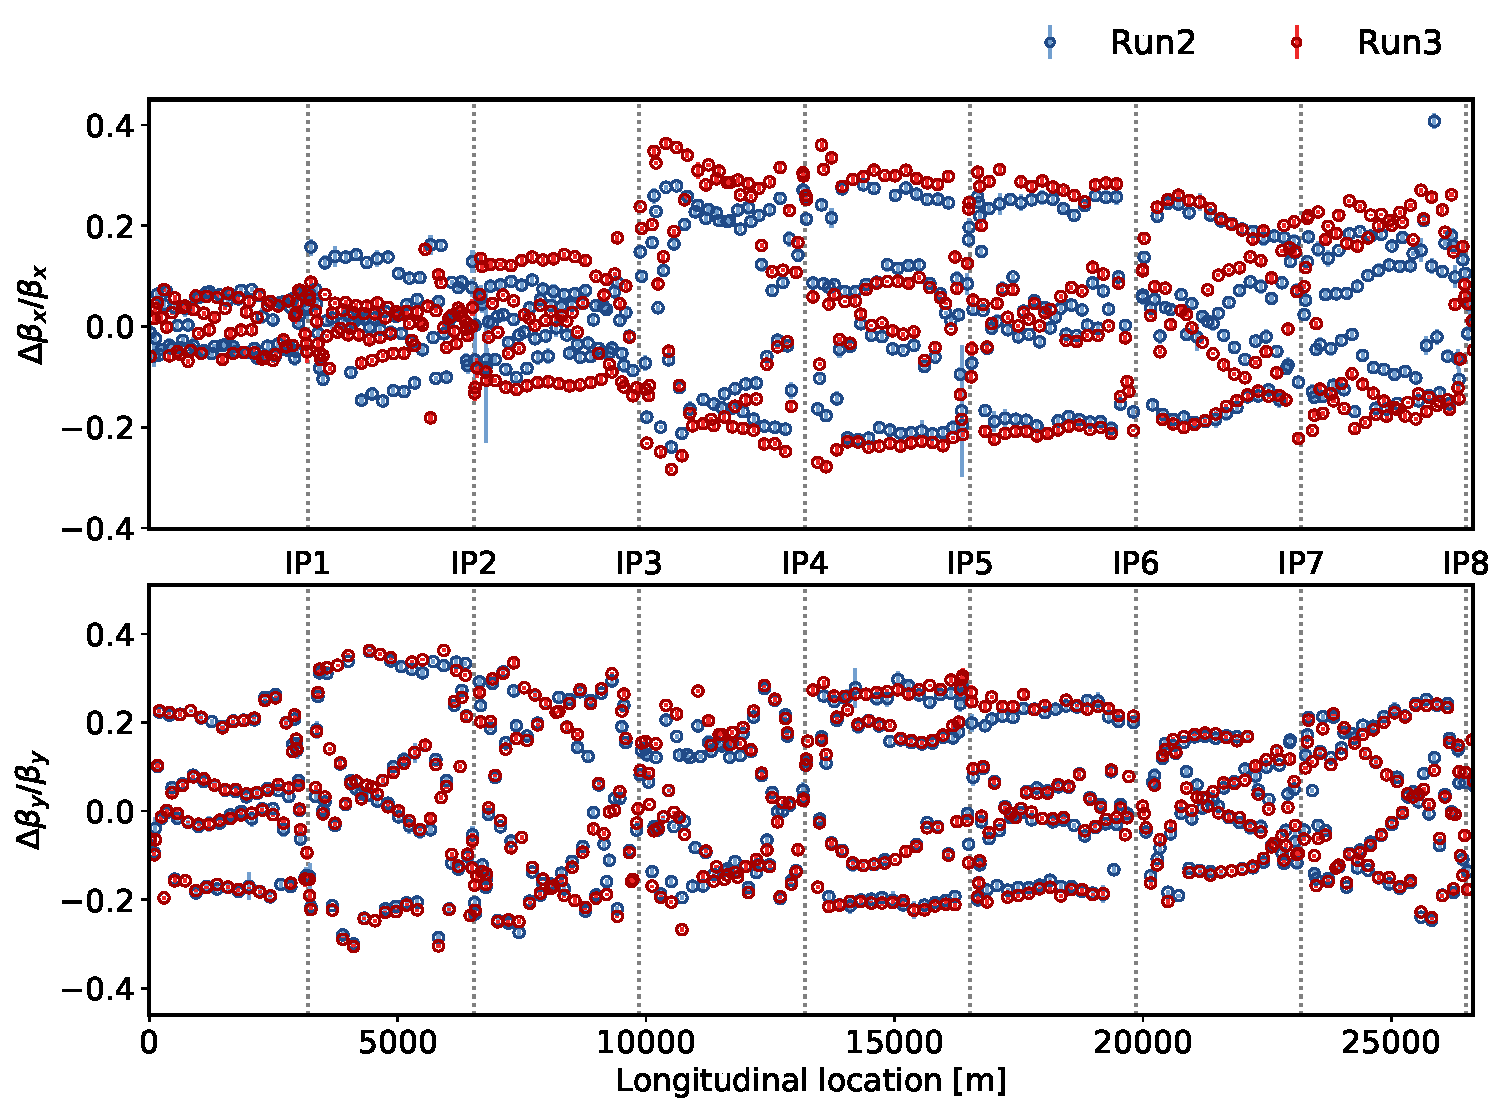
\includegraphics[width=.8\linewidth]{plots/beam2/B2_BetaBeat_afterIR3Q7fix_vs_virgin2016.pdf}  
  \caption{Beam~2}
  \label{fig:sub-second}
\end{subfigure}
\caption{After fix of swap of IR3Q7 vs 2016 virgin.}
\label{fig:after_swap_vs_2016}
\end{figure}

Based on the measurement after the correction of the swapped quadrupole a correction of the phase advance as well as the normalized dispersion was calculated. The impact on the $\beta$-beat is shown in Fig.~\ref{fig:before_after_correction_beta_beat} and the impact on the normalized dispersion is shown in Fig.~\ref{fig:before_after_correction_beta_beat}. The result is well within the required machine protection limit and similar to what has been measured as $\beta$-beat in the past. 


\begin{figure}[ht]
\begin{subfigure}{.5\textwidth}
  \centering
  % include first image
  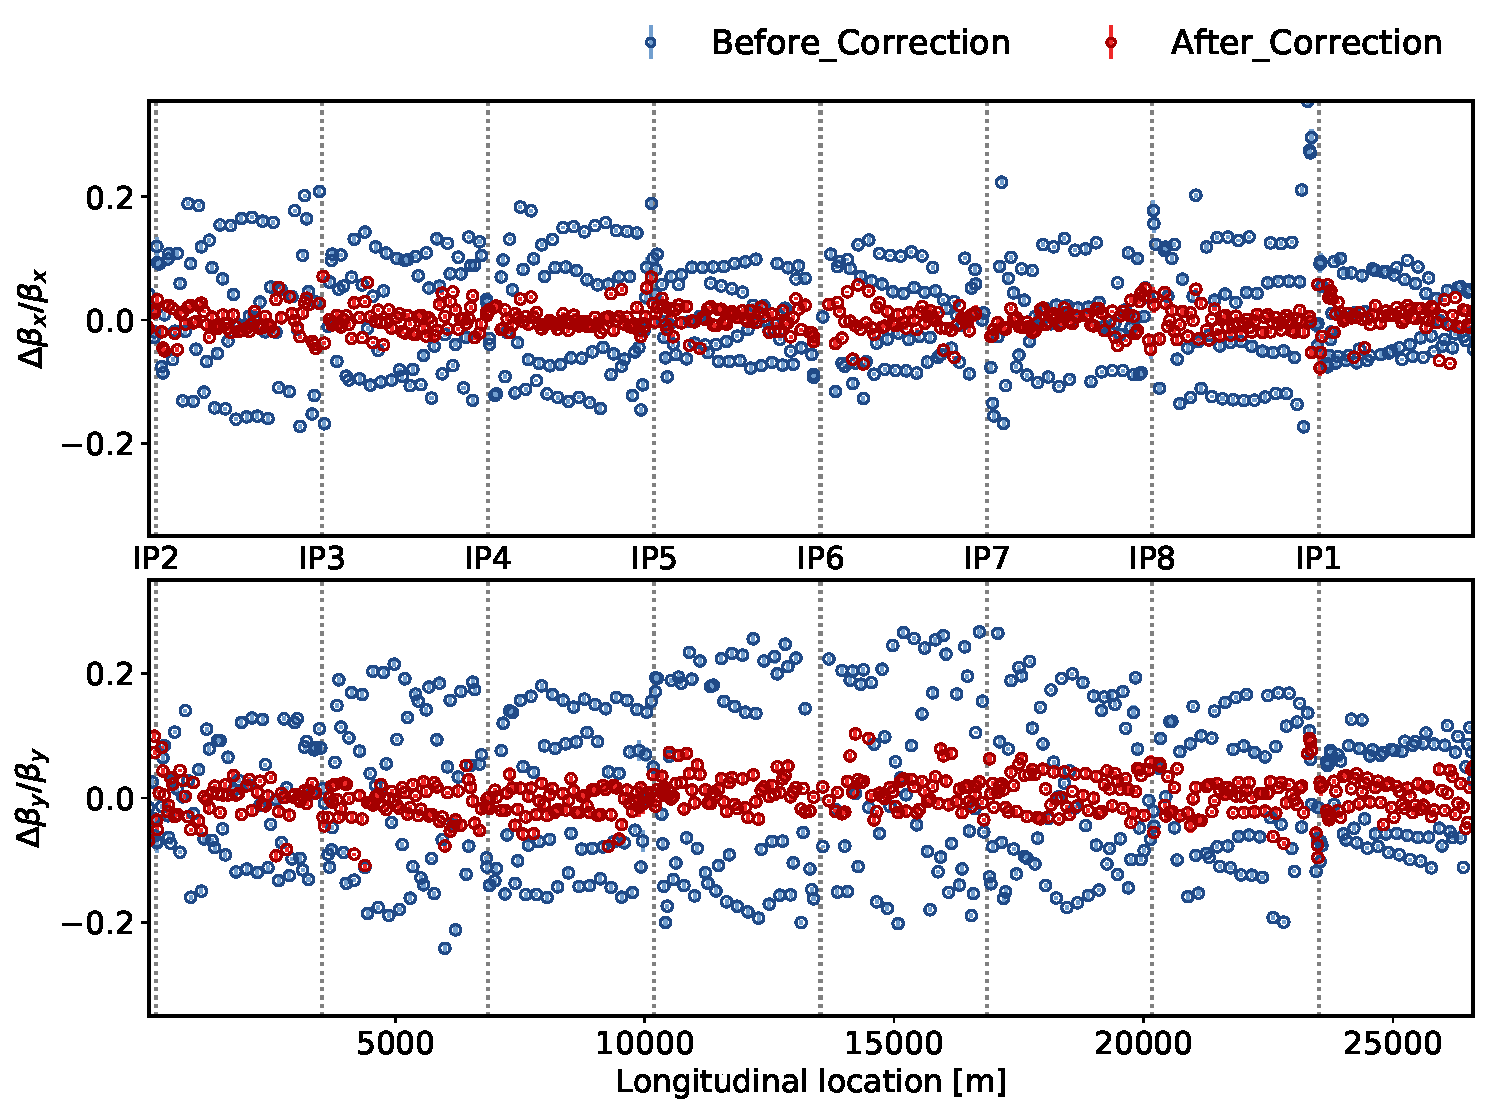
\includegraphics[width=.8\linewidth]{plots/beam1/beta_beat_before_and_after_corr.pdf}  
  \caption{Beam~1}
  \label{fig:sub-first}
\end{subfigure}
\begin{subfigure}{.5\textwidth}
  \centering
  % include second image
  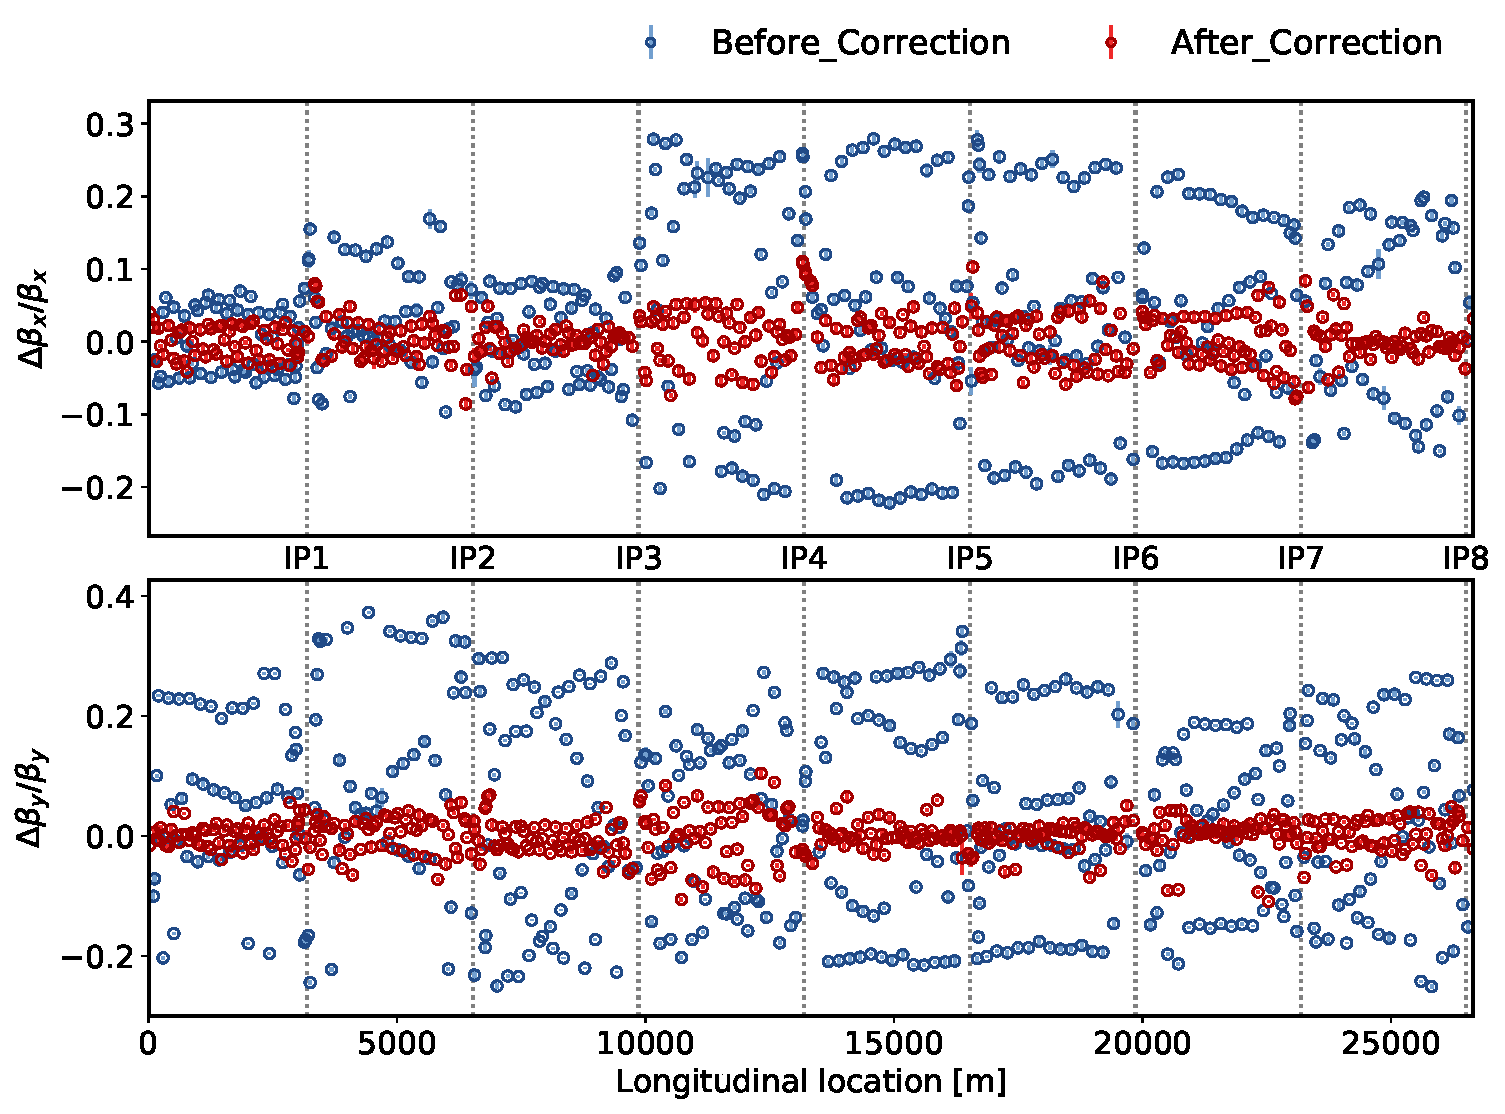
\includegraphics[width=.8\linewidth]{plots/beam2/beta_beat_before_after_correction.pdf}  
  \caption{Beam~2}
  \label{fig:sub-second}
\end{subfigure}
\caption{Beta-beat before and after correction.}
\label{fig:before_after_correction_beta_beat}
\end{figure}

\begin{figure}[ht]
\begin{subfigure}{.5\textwidth}
  \centering
  % include first image
  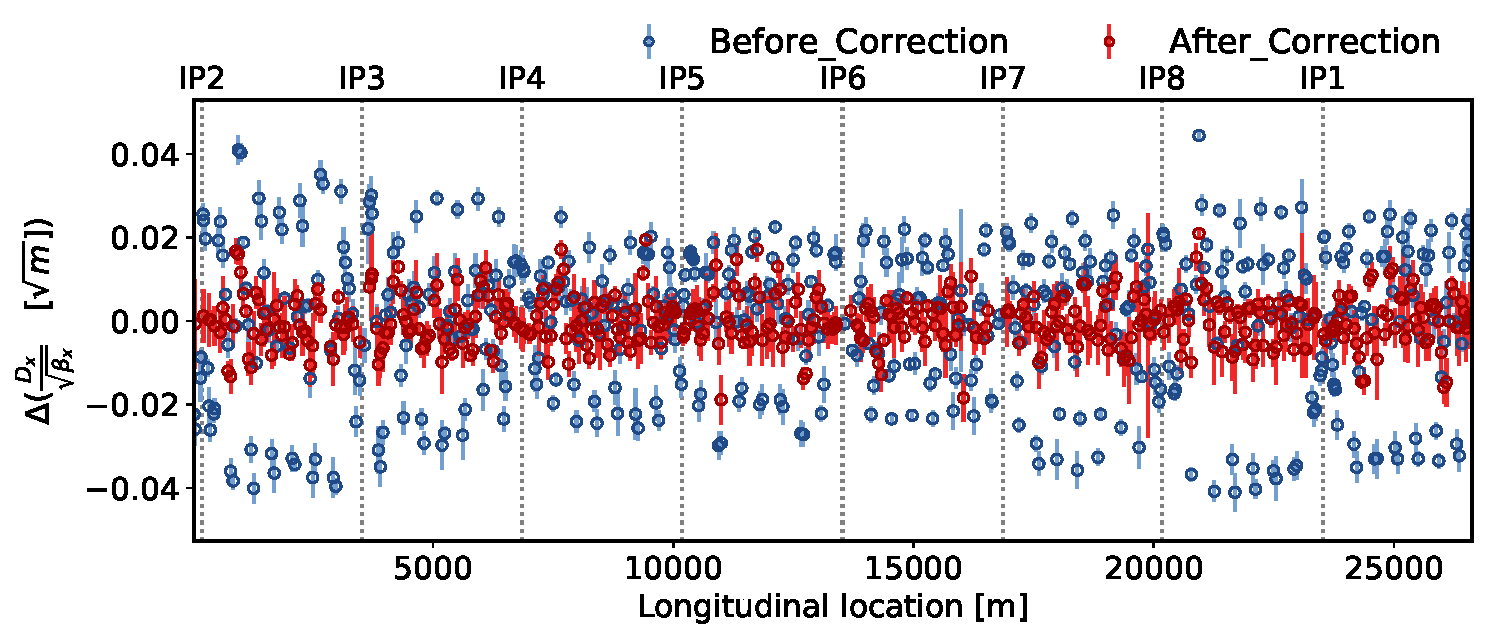
\includegraphics[width=.8\linewidth]{plots/beam1/Normalized_disp_before_vs_after_corection.pdf}  
  \caption{Beam~1}
  \label{fig:sub-first}
\end{subfigure}
\begin{subfigure}{.5\textwidth}
  \centering
  % include second image
  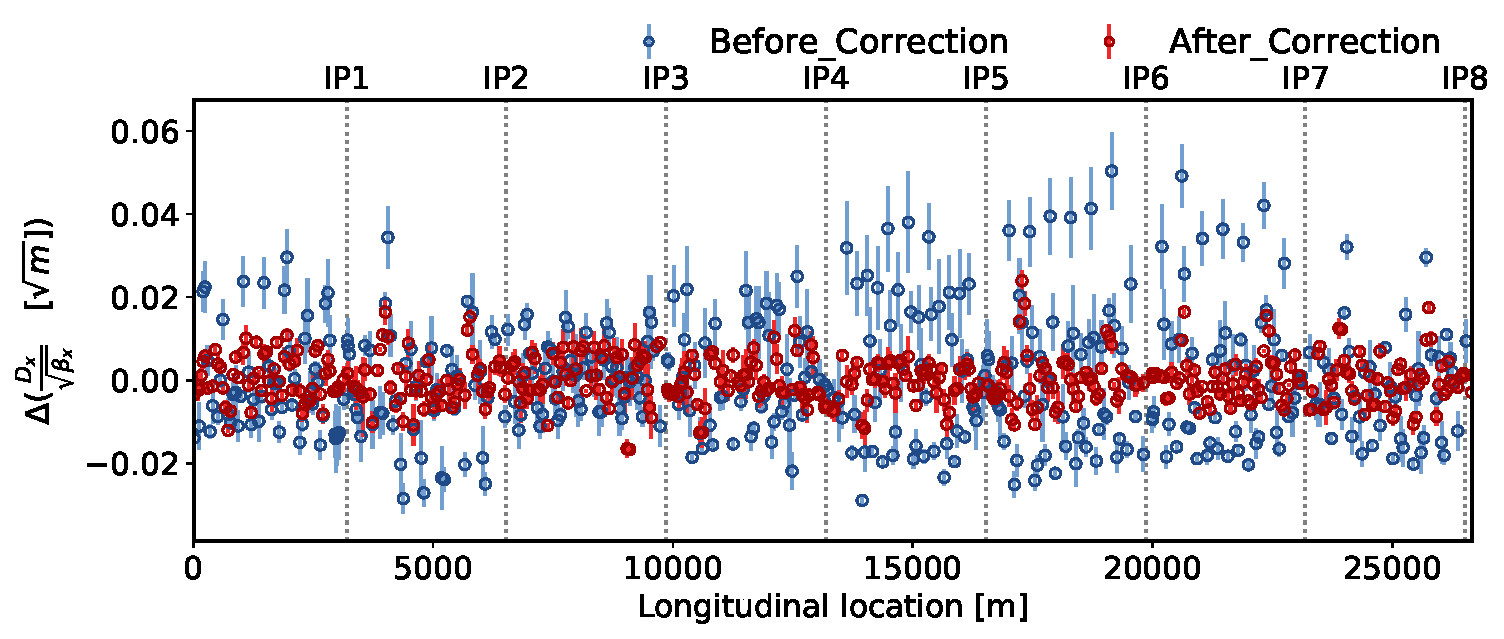
\includegraphics[width=.8\linewidth]{plots/beam2/ndisp_before_after_correction.pdf}  
  \caption{Beam~2}
  \label{fig:sub-second}
\end{subfigure}
\caption{Normalized dispersion before and after correction.}
\label{fig:before_after_correction_beta_beat}
\end{figure}

\subsection{After correction}
It is also interesting to observe if we were correcting to the same level as in Run2. 

\clearpage
\section{Q'' and Q''' measurements}

Two attempts were made during the beam-test to measure the chromaticity. The first attempt was successful while the second one only was a half scan, resulting in non exploitable data. Moreover, corrections were done for this second measurement assuming last run's values.\\
The times below are local times.

\begin{longtable}[h]{l l}
  \toprule
  \textbf{Beam Process}: & SPOOLS-6.8TeV-2021\_V1@0\_[START]\\
  \textbf{Date}: & 2021-10-22 \\
  \textbf{Start Time}: & 16:05:30\\
  \textbf{End Time}: & 16:37:00\\
  \textbf{dpp range:} & -0.0027 to +0.0017 \\
  \bottomrule
  \caption{First Measurement}
\end{longtable}

\begin{longtable}[h]{l l}
  \toprule
  \textbf{Beam Process}: & SPOOLS-6.8TeV-2021\_V1@0\_[START]\\
  \textbf{Date}: & 2021-10-31\\
  \textbf{Start Time}: & 12:16:00\\
  \textbf{End Time}: & 12:30:00 \\
  \textbf{dpp range:} & -0.0033 to +0.00\\
  \midrule
  \textbf{MCO Strengths}: & B1/B2: +3.9 / +2.7 \\
  \textbf{MCD Strengths}: & B1/B2: +2316 / +2053 \\
  \bottomrule
  \caption{Second Measurement}
\end{longtable}

% Plots for Beam 1, first axis X, then Y
\begin{figure}[H]
  \centering
  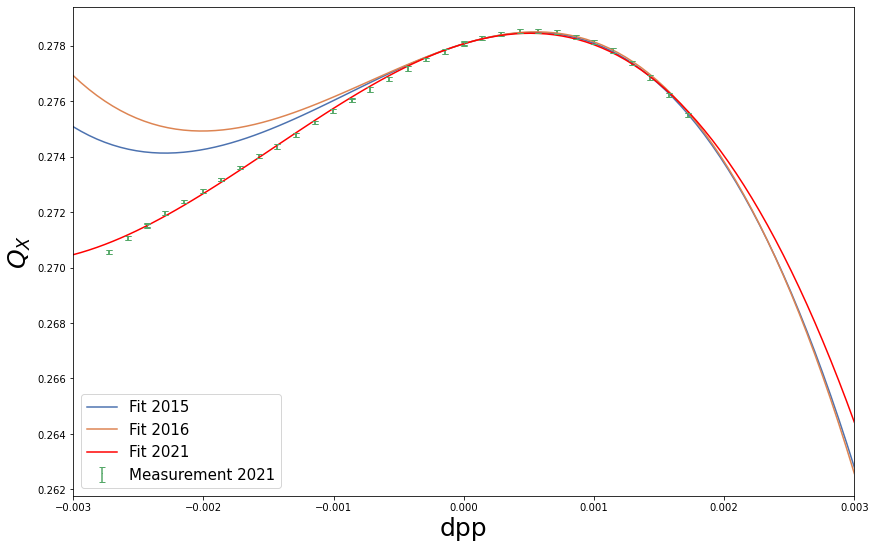
\includegraphics[width=.8\linewidth]{plots/beam1/qxb1.png}  
  \caption{Chromaticity on the X axis for Beam 1}
\end{figure}
\begin{figure}[H]
  \centering
  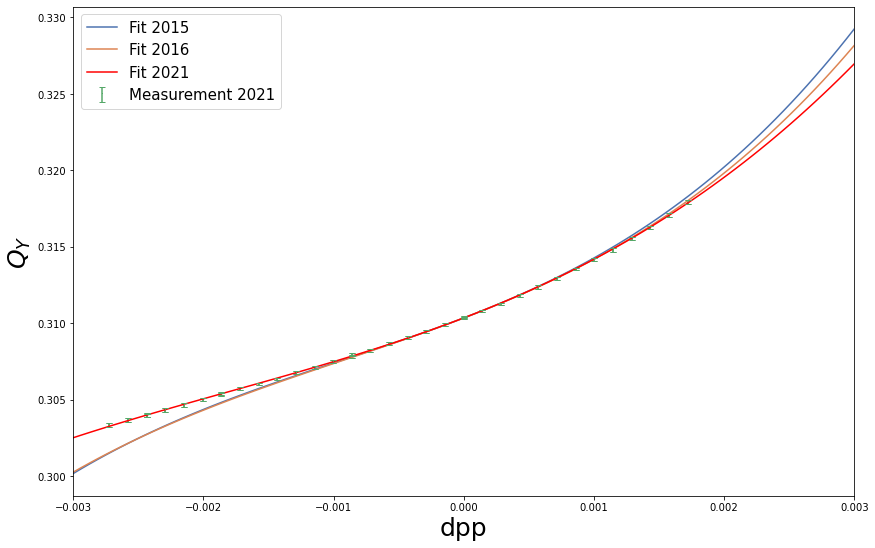
\includegraphics[width=.8\linewidth]{plots/beam1/qyb1.png}  
  \caption{Chromaticity on the Y axis for Beam 1}
\end{figure}

% Plots for Beam 2, first axis X, then Y
\begin{figure}[H]
  \centering
  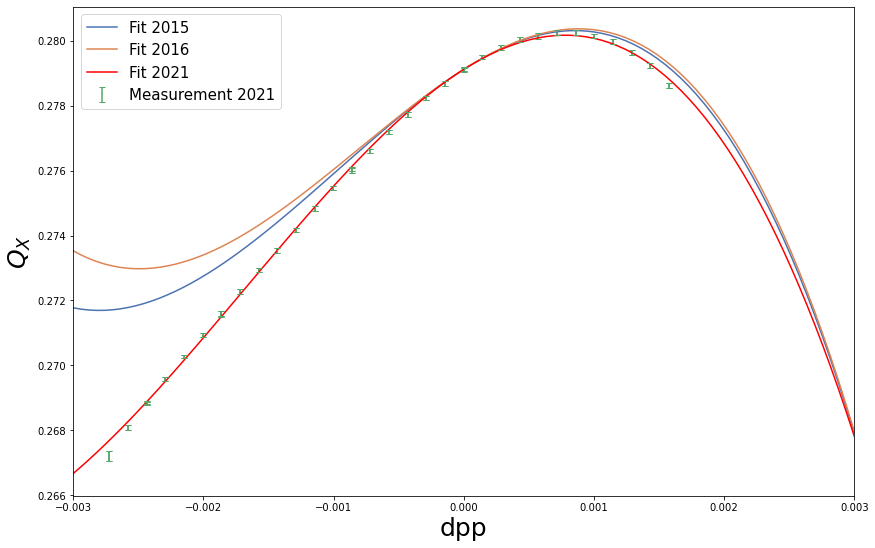
\includegraphics[width=.8\linewidth]{plots/beam2/qxb2.png}  
  \caption{Chromaticity on the X axis for Beam 2}
\end{figure}
\begin{figure}[H]
  \centering
  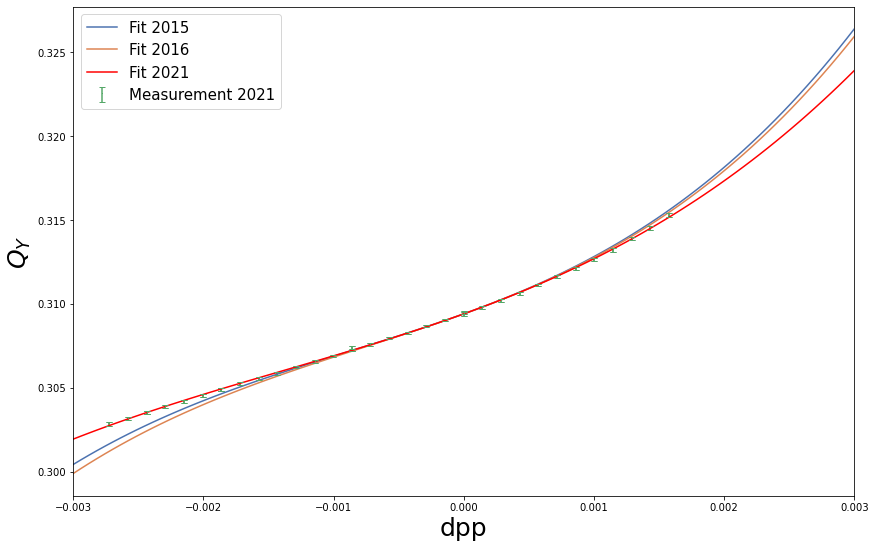
\includegraphics[width=.8\linewidth]{plots/beam2/qyb2.png}  
  \caption{Chromaticity on the Y axis for Beam 2}
\end{figure}

\begin{longtable}[h]{@{}l|c|rr|rr@{}}
  \toprule
  Year & Beam & $Q_x''[10^3]$ &   $Q_x'''[10^6]$ &   $Q_y''[10^3]$ &  $Q_y'''[10^6]$ \\
  \midrule
  \endhead
  2011 &   B1 &   $-1.8 \pm 0.03$ &  $-2.2 \pm 0.1$ &   $0.86 \pm 0.02$ &   $0.73 \pm 0.07$ \\
       &   B2 &   $-1.7 \pm 0.05$ &  $-1.1 \pm 0.1$ &   $0.82 \pm 0.02$ &   $0.90 \pm 0.06$ \\
  \midrule
  2015 &   B1 &   $-2.03 \pm 0.02$ &  $-2.31 \pm 0.08$ &   $0.97 \pm 0.02$ &   $1.06 \pm 0.04$ \\
       &   B2 &   $-2.06 \pm 0.02$ &  $-2.12 \pm 0.05$ &   $0.89 \pm 0.01$ &   $1.02 \pm 0.02$ \\
  \midrule
  2016 &   B1 &   $-1.85 \pm 0.03$ &  $-2.54 \pm 0.07$ &   $0.86 \pm 0.01$ &   $0.93 \pm 0.04$ \\
       &   B2 &   $-1.86 \pm 0.02$ &  $-2.31 \pm 0.05$ &   $0.78 \pm 0.01$ &   $1.03 \pm 0.05$ \\
  \midrule
  2021 &   B1 &   $-2.36 \pm 0.03$ &  $-1.62 \pm 0.04$ &  $0.98 \pm 0.01$ &  $0.55 \pm 0.02$ \\
       &   B2 &   $-2.64 \pm 0.03$ &  $-1.56 \pm 0.05$ &  $0.78 \pm 0.01$ &   $0.58 \pm 0.02$ \\
  \bottomrule
  \caption{Non Linear Chromaticity Results and History}
\end{longtable}

\section{3D kicks}

\section{MCS feed-down}
It has been observed that changing the strength of the MCS ($b_3$ spool pieces) have an impact on the transverse coupling in the LHC. The main hypothesis is that this is coming from a vertical misalignment of the MCS. In order to validate if the effect had remained constraint after the Long Shutdowns a new measurement was carried out during the beam-test. The result for Beam~1 is showin in Fig.~\ref{}

\begin{figure}[ht]
\begin{subfigure}{.5\textwidth}
  \centering
  % include first image
  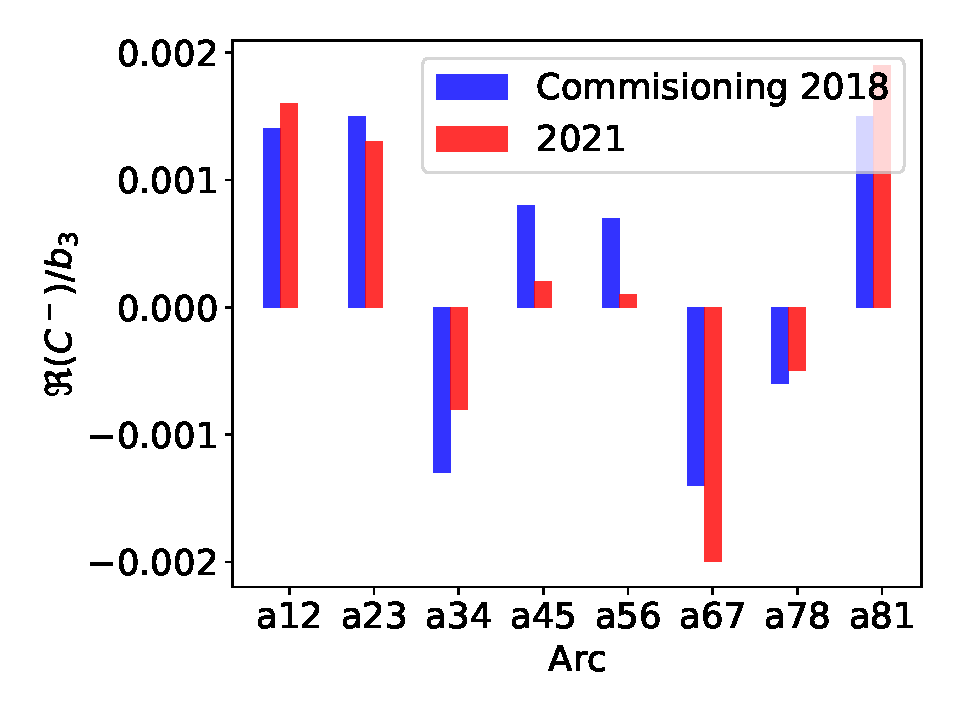
\includegraphics[width=.8\linewidth]{plots/MCS/b_1change_re_per_b3.pdf}  
  \caption{Real part of the $C^-$. }
  \label{fig:sub-first}
\end{subfigure}
\begin{subfigure}{.5\textwidth}
  \centering
  % include second image
  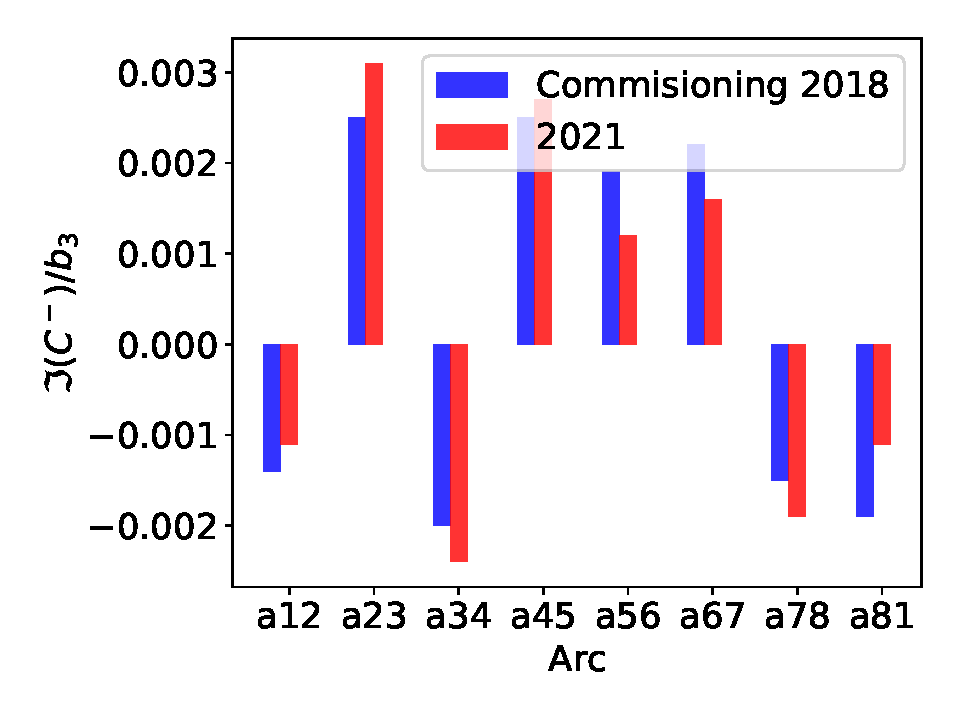
\includegraphics[width=.8\linewidth]{plots/MCS/b_1change_im_per_b3.pdf}  
  \caption{Imaginary part of the $C^-$.}
  \label{fig:sub-second}
\end{subfigure}
\caption{Beta-beat before and after correction.}
\label{fig:fig}
\end{figure}

\begin{figure}[ht]
\begin{subfigure}{.5\textwidth}
  \centering
  % include first image
  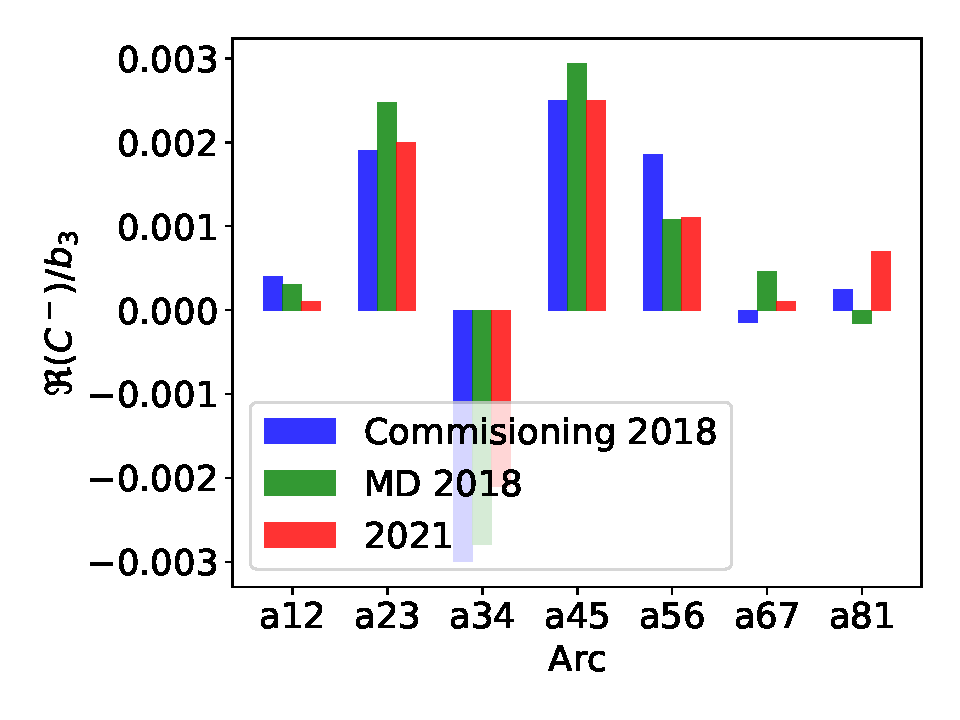
\includegraphics[width=.8\linewidth]{plots/MCS/b2_change_re_per_b3.pdf}  
  \caption{Real part of the $C^-$.}
  \label{fig:sub-first}
\end{subfigure}
\begin{subfigure}{.5\textwidth}
  \centering
  % include second image
  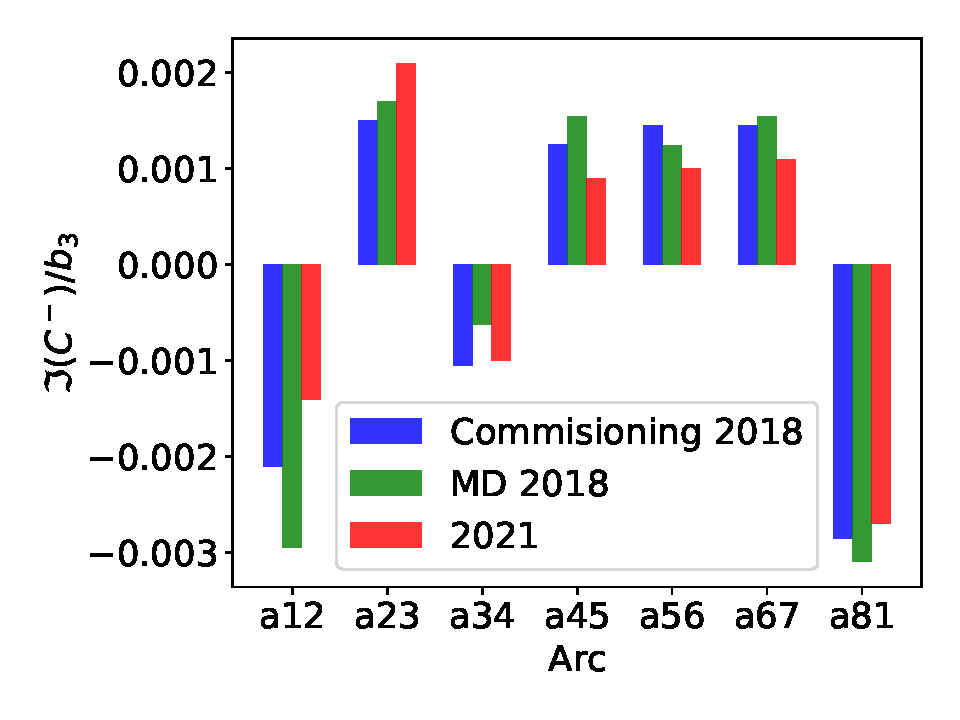
\includegraphics[width=.8\linewidth]{plots/MCS/b_2change_im_per_b3.pdf}  
  \caption{Imaginary part of the $C^-$.}
  \label{fig:sub-second}
\end{subfigure}
\caption{}
\label{fig:fig}
\end{figure}

\section{Additional observations}
All

\section{Summary and Outlook}
The optics corrections during the beam test was very successful in terms of demonstrating the readiness of the optics corrections tools as well as finding the swap of the magnet RRR. Furthermore, it 

\begin{thebibliography}{99}   % Use for  1-9  reference
\end{thebibliography}
\appendix
\section{Decay compensation}
Based on the measurement of the feed-down from the MCS to coupling a new powering to compensate for the b3 decay in the dipoles have been calculated. It is matched in such a way that it compensates the chromaticity by the same amount as the even compensation but distributed in such a way that the coupling is expected to stay constant. The knobs for this are the following:
\begin{verbatim}

RCS.A12B1/K2 0.8630127907663837 
RCS.A23B1/K2 0.779866457813889 
RCS.A34B1/K2 1.3828734821095998 
RCS.A45B1/K2 0.4445174033278492 
RCS.A56B1/K2 0.9114975331776818 
RCS.A67B1/K2 1.401218693590656 
RCS.A78B1/K2 1.3540008484475567 
RCS.A81B1/K2 0.8630127907663839 

RCS.A12B2/K2 0.6866554457561092 
RCS.A23B2/K2 0.9619053275562472 
RCS.A34B2/K2 1.5867931783979445 
RCS.A45B2/K2 0.7923501971731068 
RCS.A56B2/K2 0.9643136781336532 
RCS.A67B2/K2 1.391600462298758 
RCS.A78B2/K2 1.16296351210475 
RCS.A81B2/K2 0.5945946691676663 

\end{verbatim}
\end{document}
